\begin{figure}[t]
\centering
    \begin{minipage}{0.47\textwidth}
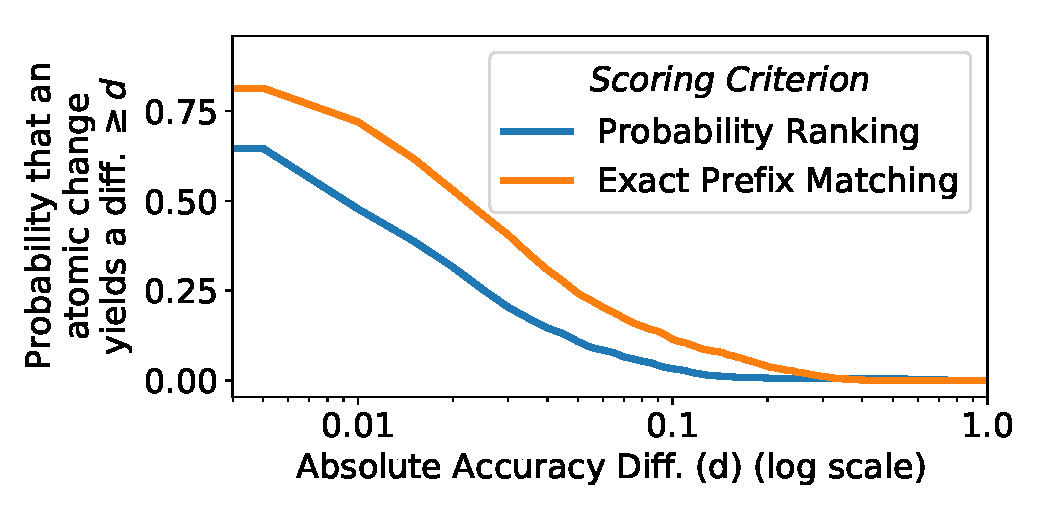
\includegraphics[width=\linewidth]{figures/edges_weights_with_both_scoring.pdf}
    \caption{Probability that an atomic change (e.g. changing a space, separator) has a given impact in accuracy for two scoring criteria. \tbdone{53} tasks, 30 sampled atomic changes each.} \label{fig:edge_probability}
    \end{minipage}\hfill
\begin{minipage}{0.47\textwidth}
  \centering
  %\begin{subfigure}[t]{0.01\linewidth}
  %  \textbf{a.}
  %\end{subfigure}
%  \begin{subfigure}[t]{0.4\linewidth}
    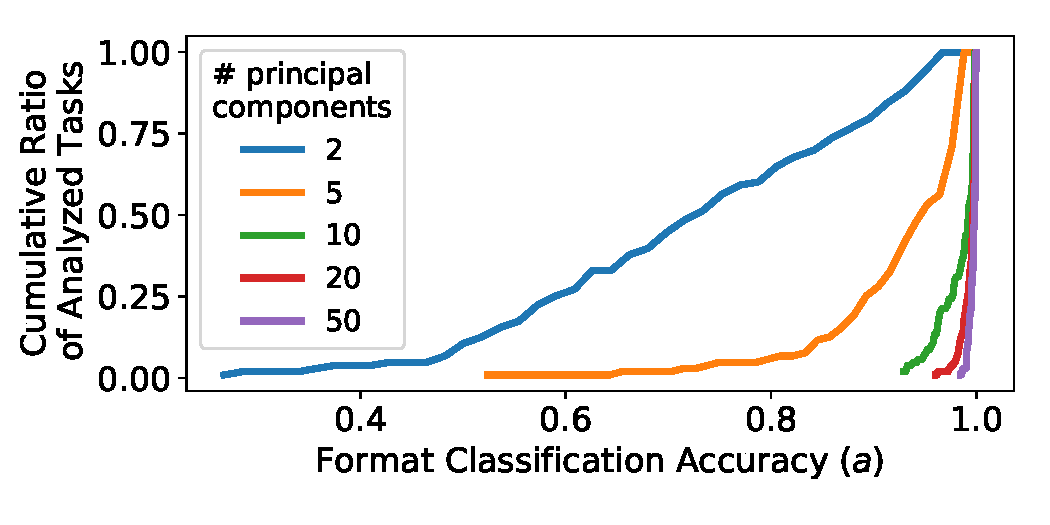
\includegraphics[width=\linewidth, valign=t]{figures/pca_classification_cumulative_distribution_across_nshots.pdf}
    \caption{Cumulative ratio of tasks that can be classified with at most $a$ accuracy using the top principal components of the last decoding layer of the prompt. %Using the top 50 principal components all formats are classified with $>.99$ accuracy.
    } \label{fig:pca}
%  \end{subfigure}\hfill
%\caption{\textit{Prompt formats are identifiable transformations of the output probability distribution.}}
\end{minipage}
\vspace{-3mm}
\end{figure}
